

\section{\model{} Architecture}
\label{sec: method}

H-Nets are defined as hierarchical U-Net-like networks, but with data-dependent \emph{dynamic subsampling} that is learned end-to-end together with the rest of the model.
We first introduce H-Net's hierarchical architecture for multi-level processing, establishing key design principles (\cref{sec: Method-Architectural-Overview}).
We then present our dynamic chunking mechanism that learns content-aware compression through standard optimization (\cref{sec: Method-Dynamic-Chunking-Mechanism}).
Next, we detail architectural and optimization enhancements specifically tailored for hierarchical sequence modeling (\cref{sec: Improved-Techniques}).
Finally, we explain how H-Net preserves autoregressive properties throughout its hierarchical structure during both training and inference (\cref{sec: Method-Autoregressive-Training-and-Inference}).

\subsection{Architectural Overview}
\label{sec: Method-Architectural-Overview}

\subsubsection{Components of \model{}}

\model{} employs a hierarchical architecture comprising three primary components -- \encoder{s} ($\mathcal{E}$), \main{} ($\mathcal{M}$), and \decoder{s} ($\mathcal{D}$)  -- where each component is implemented with a stack of sequence mixing layers (\eg{} Transformers or state space models).
In its simplest form, a single-stage \model{} consists of one \encoder{}, one \main{}, and one \decoder{}.
Crucially, the architecture's key characteristic lies in the \main{}'s unique property: it can itself be instantiated as a complete \model{}, enabling recursive construction of multi-level hierarchies.

This recursive design allows \model{} to scale to arbitrary depths.
In an $S$-stage model, we denote components at each stage using superscripts: \encoder{s} as $\mathcal{E}^s$ and \decoder{s} as $\mathcal{D}^s$ for stages $0 \leq s < S$, with the \main{} $\mathcal{M}$ residing only at the final stage $s=S$.
For example, a two-stage model contains $\mathcal{E}^0$, $\mathcal{E}^1$, $\mathcal{M}$, $\mathcal{D}^1$, and $\mathcal{D}^0$, as illustrated in \cref{fig: main}-(Left).
Throughout this paper, we use superscripts to denote stage indices, though we omit them when all variables within an equation belong to the same stage.

Drawing inspiration from the U-Net architecture~\citep{U-Net}, \model{} progressively compresses input sequences into fewer vectors with richer semantic embeddings through a \chunk{}, processes these representations in the \main{}, then decompresses the sequence back to its original resolution using a \dechunk{}.
Unlike traditional U-Net designs, however, \model{} dynamically determines chunking boundaries rather than using fixed-size pooling operations.
The overall pipeline can be formalized as:

\begin{equation}
    \label{eq: stages}
    \hat{x}^{s} = \mathcal{E}^{s}(x^{s}), \qquad\qquad \hat{z}^S = \mathcal{M}(x^S), \qquad\qquad \hat{z}^{s} = \mathcal{D}^{s}(z^{s}),
\end{equation}

where the \chunk{} and the \dechunk{} operations are defined as:

\begin{minipage}[t]{.45\linewidth}
  \begin{equation}
    \label{eq: tokenizer}
    (x^{s+1},\space p^{s}) = \mathsf{Chunk}(\hat{x}^s),
  \end{equation}
\end{minipage}
\begin{minipage}[t]{.55\linewidth}
  \begin{equation}
    \label{eq: detokenizer}
    z^{s} = \mathsf{Dechunk}(\hat{z}^{s+1}, p^{s}) + \mathsf{Linear}(\hat{x}^{s}).
  \end{equation}
\end{minipage}



The initial input to the model is $x^0 \in \mathbb{R}^{L^0 \times D^0}$ where $L^0$ is the input sequence length and $D^0$ is the embedding dimension.
Intuitively, $p^{s} \in [0,1]^{L^s}$ represents the chunking router's confidence that the token should be passed into the main stage.
\footnote{We also sometimes refer to it as a \emph{probability}---it is interpreted as such in \cref{sec: distill}---although we do not use it as a formal probability.}
This value is essential for both the chunk (\cref{sec: tokenizer}) and dechunk operations (\cref{sec: detokenizer}).

\subsubsection{Design Principles}

\paragraph{Encoder and Decoder Networks.}
The encoder and decoder networks in \model{} face unique design constraints due to their dual objectives and computational requirements.
Each encoder must simultaneously (i) preserve fine-grained information for transmission to its corresponding decoder through residual connections \eqref{eq: detokenizer}, and (ii) compress inputs into chunks of richer representations for the \main{}.
The decoder, in turn, must effectively combine coarse-grained representations from the \main{} with fine-grained details from the encoder residuals.

Importantly, both encoders and decoders operate on uncompressed sequences, making computational efficiency a significant design constraint that shapes our architectural choices.
Recent studies demonstrate that state space models (SSMs)~\citep{S4, Mamba} excel at processing fine-grained data including audio~\citep{SaShiMi}, DNA sequences~\citep{Caduceus}, and robotic control signals~\citep{ssm-rl}.

Based on these insights, we employ Mamba-2 layers~\citep{Mamba2} as the primary building blocks for the encoder and decoder networks.
This choice yields two significant benefits: effective handling of fine-grained inputs, and substantially improved efficiency when processing long, uncompressed sequences.
Our ablation studies (\cref{sec: ablation_studies}) confirm that SSM-based encoders/decoders significantly outperform Transformer layers,
not just at the byte level but even on coarser inputs, which we attribute to their stronger inductive bias for compression which helps build abstractions~\citep{gu2025tradeoffs}.

\paragraph{Main Network.}

\model{}'s computational efficiency stems from strategic parameter allocation.
We concentrate the majority of model capacity in the \main{}, which operates on progressively compressed sequences.
After $S$ stages of compression, the \main{} receives sequences where $L^S \ll L^0$, enabling much larger networks within the same computational budget.
This design reflects two key principles: (i) compressed sequences allow more parameters and compute per chunk, and (ii) higher-level abstractions benefit from increased processing power.

The \main{} functions as a standard language model and can employ any sequence mixing architecture.
We default to Transformer layers for two reasons: compressed representations align well with Transformers' strengths in processing discrete, semantically-rich tokens, and this choice enables more controlled comparison with traditional BPE-based Transformer baselines in our experiments.
However, the modular design also allows straightforward substitution with alternative architectures (\eg{} a state space model, hybrid,  or \model{} itself) as explored in our ablations.

\paragraph{Architectural Guidelines.}
Compared to standard isotropic models, the H-Net's structure introduces several new dimensions of architectural parameters to balance the parameter/compute allocation to each network.
To simplify the search space, we follow a few general guidelines.
\begin{itemize}
    \item  First, we ensure the model width (often referred to as $d_{\text{model}}$ for isotropic architectures) is monotone in the hierarchy: $D^0 \leq D^1 \leq \dots \leq D^S$.
    This allows increasing compute and parameters used in the main network without significantly increasing its depth.
    \item Second, using efficient and powerful SSM layers in the outer networks allow reducing the number of layers used compared to similar prior architectures that only used Transformer layers~\citep{SpaceByte};
    in this paper, we always stick to four layers (or the equivalent of four Mamba layers) in each encoder/decoder network.
\end{itemize}
To handle the changes in dimensions without an additional linear layer, we adopt the technique used in SpaceByte~\citep{SpaceByte} with the marginal change: to expand dimensions (\ie{} $D^{s} \rightarrow D^{s+1}$), we append all vectors with a shared trainable vector of dimension $D^{s+1}-D^{s}$; to reduce dimensions (\ie{} $D^{s+1} \rightarrow D^{s}$), we take the first $D^{s}$ dimensions from each vector.

We note that H-Net's performance can likely be improved with more careful tuning of the layer allocation and hyperparameters between sub-networks.


\subsection{Dynamic Chunking (DC)}
\label{sec: Method-Dynamic-Chunking-Mechanism}

\model{} learns chunking boundaries through end-to-end training, allowing it to identify semantically meaningful units adaptively.
Furthermore, this dynamic approach enables the model to allocate computational resources efficiently by compressing low-information regions while preserving high-information content at appropriate granularity.

\subsubsection{\CHUNK{}}
\label{sec: tokenizer}
The \chunk{} ($\mathsf{Chunk}$ in equation \eqref{eq: tokenizer}) contains a \router{} and \downsampler{}, as illustrated in \cref{fig: main}-(\colorbox{Chunk}{bottom-right}).

\paragraph{\ROUTER{}.}
In natural data, meaningful boundaries tend to emerge at points of contextual or semantic shift.
From this observation, we add an inductive bias by measuring the similarity between adjacent representations: when context changes, consecutive vectors should exhibit lower similarity.
The \router{} implements this intuition through cosine similarity between adjacent encoder outputs.
Given encoder outputs $\hat{X}$, it calculates boundary probabilities $p_t$ and boundary indicators $b_t$ as follows:

\begin{equation}
\label{eq: Rounting-Module}
q_t = W_q \hat{x}_t, \quad k_t = W_k \hat{x}_t, \qquad p_t = \frac{1}{2} \left(1 - \frac{q_t^\top k_{t-1}}{\left\Vert q_t \right\Vert \left\Vert k_{t-1} \right\Vert}\right) \in [0, 1], \quad b_t = \mathds{1}_{\{p_t \geq 0.5\}},
\end{equation}
where $p_1 = 1.0$ by definition, ensuring the sequence begins with a boundary.
This formulation scales cosine similarity into a boundary score or probability: ideally, when consecutive vectors $\hat{x}_{t-1}$ and $\hat{x}_t$ span a semantic boundary (\eg{} between morphemes, words, or phrases), their projections $q_t$ and $k_{t-1}$ diverge in the latent space, yielding low cosine similarity and consequently high boundary probability $p_t$.

\paragraph{\Downsampler{}.}
The \downsampler{} compresses encoder outputs $\hat{x}^s$ into a reduced set of vectors $x^{s+1}$ using boundary indicators $\{b_t^s\}_{t=1}^{L^s}$.
Among potential compression strategies -- including mean pooling, max pooling, or cross-attention -- we adopt direct selection of boundary-marked vectors for its simplicity and effectiveness (see \cref{sec: Appendix-Various-Compression} for ablations).

As illustrated in \cref{fig: main}-(b), this approach follows a straightforward selection rule: vectors where $b_t = 1$ are retained in the compressed sequence $x^{s+1}$, while those where $b_t = 0$ are discarded.
Likewise, the same \downsampler{} applies to boundary probabilities, compressing $p^s$ into $P^{s+1}$ for use in a \dechunk{} (see \cref{sec: detokenizer}).

\subsubsection{Dechunking}
\label{sec: detokenizer}

The \dechunk{} ($\mathsf{Dechunk}$ in equation \eqref{eq: detokenizer}) consists of a \smoother{} and \upsampler{}, as illustrated in \cref{fig: main}-(\colorbox{DeChunk}{top-right}).

\paragraph{\SMOOTHER{}.}
The critical challenge in training a dynamic chunking module lies in the discrete nature of chunk boundaries, which impedes gradient flow during backpropagation.
We introduce the smoothing module as a technique to address this problem.
As illustrated in \cref{fig: main}-(c), this component transforms discrete chunking operations into differentiable computations by creating smooth interpolations between chunks.
Concretely, the \smoother{} applies an exponential moving average (EMA) with the following definition:
\begin{equation}
    \label{eq: ema}
    \bar{z}_t = P_t \hat{z}_t + (1-P_t) \bar{z}_{t-1}.
\end{equation}

\begin{figure}[t!]
    \centering
    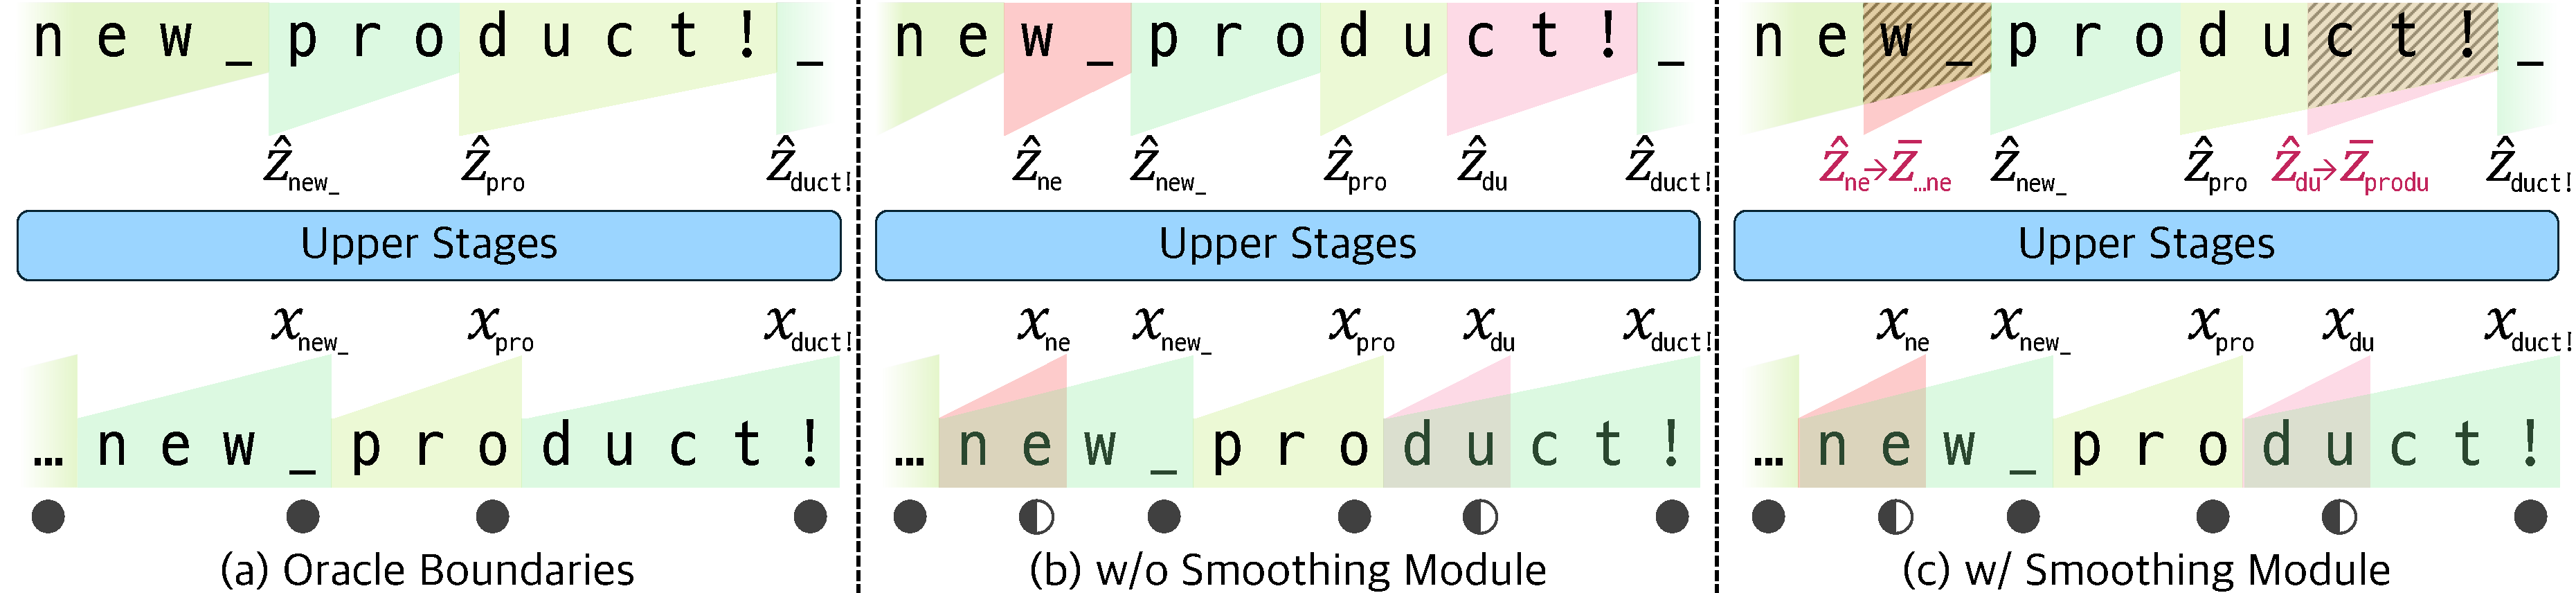
\includegraphics[width=1.0\linewidth]{fig_img/new_product.pdf}
    \caption{
    Comparison of decompression strategies on the example sequence \texttt{"...new product!"}.
    $\CIRCLE$ indicates a boundary with high confidence ($P_t=1.0$) and $\LEFTcircle$ indicates a boundary with low confidence ($P_t=0.5$).
    As each letter in the example is unique, we use the letters in subscripts to denote expected semantics of chunks.
    (a) Optimal chunking with oracle boundaries identifying linguistically meaningful units.
    (b) Suboptimal chunking without a \smoother{}.
    This creates misalignment during upsampling, causing information from incorrect contexts to propagate.
    (c) Improved decompression with a \smoother{}, where low-confidence chunks are interpolated with weighted combinations of previous chunks, correcting the shaded regions.
    In panels (b) and (c), we interpret low-confidence boundaries cause the encoder network to embed broader contexts at subsequent positions.
    Specifically, the vectors at \texttt{\_} and \texttt{!} encode \texttt{new\_} and \texttt{duct!}, respectively (instead of \texttt{w\_} and \texttt{ct!}).
    }
    \label{fig: new_product}
\end{figure}


Our \smoother{} performs several roles:
\begin{itemize}
    \item \textbf{Differentiable boundary learning:} It transforms the discrete upsampling operation into a continuous one, enabling effective backpropagation through chunk boundaries during training without requiring stochastic exploration-based approaches~\citep{GumbelSoftmax}.
    \item \textbf{Adaptive error correction:} Chunks with high confidence ($P_t \approx 1.0$) maintain discrete boundaries ($\bar{z}_t \approx z_t$), while chunks with low confidence ($P_t \approx 0.5$) are smoothed using information from previous chunks, creating a self-correcting mechanism.
    \item \textbf{Training stability:} By smoothly interpolating between discrete choices based on confidence scores, a \smoother{} prevents the model from overfitting to suboptimal chunking patterns early in training.
\end{itemize}

\cref{fig: new_product} illustrates this with the example \texttt{"...new product!"}.
The word "product" can be morphologically decomposed into "pro-" and "-duct"\footnote{\textbf{pro-} -- meaning \emph{forward} or \emph{forth}, \textbf{-duct} -- from Latin \emph{ducere}, meaning \emph{to lead} or \emph{to bring}}.
Without the \smoother{} (see \cref{fig: new_product}-(b)), suboptimal chunking (\eg{} \texttt{"du"} as shown with half-filled circles) creates alignment mismatches that disrupt information flow.
With the \smoother{} (see \cref{fig: new_product}-(c)), chunks with low confidence are smoothed with previous context, ensuring proper information propagation and enabling the model to learn optimal chunk boundaries through gradient descent.

\paragraph{\Upsampler{}.}

We carefully design the \upsampler{} (see \cref{fig: main}-(d)) that decompresses $\bar{z}^{s+1}$ to match the original resolution of inputs in the previous stage $z^{s}$ with the following definition:

\begin{minipage}[t]{.48\linewidth}
\vspace{-3mm}
  \begin{align}
    \label{eq: coefficient}
    c_t &= p_t^{b_t} (1-p_t)^{1-b_t}
    = \begin{cases}
        p_t & \text{if } b_t=1,\\
        1 - p_t & \text{otherwise},
    \end{cases}\\
    \label{eq: STE}
    \mathsf{STE}(c_t) &= c_t + \text{stopgradient}(1-c_t),
  \end{align}
\end{minipage}\hfill
\begin{minipage}[t]{.51\linewidth}
  \begin{align}
    \label{eq: Upsampler-Upsample}
    \tilde{z}_t &= \bar{z}_{\sum_{k=1}^t b_k},\\
    \label{eq: Upsampler-Mult}
    \mathsf{Upsampler}(\bar{z}, c)_t &= \mathsf{STE}\left(c_t\right) \cdot \tilde{z}_t.
  \end{align}
\end{minipage}


Each component serves a specific purpose in enabling stable end-to-end learning:
\begin{itemize}
    \item \textbf{Confidence scoring} \eqref{eq: coefficient}: The coefficient $c$ quantifies the \router{}'s confidence in its boundary decisions.
    For positions marked as boundaries ($b_t=1$), $c_t=p_t$ rewards high boundary probabilities.
    In contrast, for non-boundary positions ($b_t=0$), $c_t=1-p_t$ penalizes false boundary predictions.
    This formulation encourages the model to produce boundary probabilities near $1.0$ at true boundaries and near $0.0$ elsewhere.
    \item \textbf{Gradient stabilization} \eqref{eq: STE}: The Straight-Through Estimator (STE)~\citep{STE} is a well established technique from discrete representation learning~\citep{VQ-VAE, GumbelSoftmax} that rounds confidence scores to $1.0$ in the forward pass while maintaining continuous gradients during backpropagation.
    While \model{} already demonstrates strong performance without STE, incorporating this technique provides an additional performance boost that empirically further stabilizes the optimization dynamics.
    \item \textbf{Causal expansion} \eqref{eq: Upsampler-Upsample}: The upsampling operation repeats each compressed vector until the next boundary position, ensuring that each reconstructed position receives information from its most recent chunk.
    This maintains the sequential flow of information while expanding the compressed representation back to its original length.
    \item \textbf{Confidence-weighted decompression} \eqref{eq: Upsampler-Mult}:
    Multiplying upsampled vectors by their confidence scores incentivizes the \router{} to make confident, accurate decisions.
    High-confidence boundaries create direct reward signals that encourage the model to sharpen its boundary predictions through gradient feedback.
\end{itemize}

\subsubsection{Ratio Loss}

Without explicit regularization, the model may converge to trivial solutions: either retaining nearly all vectors (negating computational benefits) or compressing excessively (losing critical information).
Inspired by load balancing mechanisms in Mixture-of-Experts (MoE) models~\citep{MoE}, which face similar challenges in maintaining balanced expert utilization, we introduce a ratio loss to guide compression:
\begin{equation}
    \label{eq: ratio_loss}
    \mathcal{L}_\text{ratio} = \frac{N}{N-1} \left( (N-1) FG + (1-F) (1-G) \right), \qquad F = \frac{1}{L}\sum_{t=1}^{L} b_t, \quad G = \frac{1}{L}\sum_{t=1}^{L} p_t,
\end{equation}
where $F$ represents the fraction of vectors actually selected, $G$ denotes the average boundary probability, and $N$ controls the target compression ratio.
Mechanistically, although $F$ is not differentiable, the network can be trained toward targeted compression ratios through $G$, which provides continuous feedback.

When $F = G$, the loss attains a minimum of $\mathcal{L}_\text{ratio}=1$ when $F = G = \frac{1}{N}$.
Interestingly, the loss can theoretically fall below $1$ when $F \neq G$ (\eg{} $F = \frac{1}{N} + \epsilon$ and $G = \frac{1}{N} - \epsilon$), which we indeed observe during training.
Despite this theoretical possibility, the loss effectively guides the model toward the desired compression ratio in practice.
In practice, as our architectural design encourages the \router{} to make confident decisions (\ie{} boundary probabilities approaching $0$ or $1$), $F$ naturally converges toward $G$, and the loss effectively guides the model toward the desired compression ratio.


Combined together with the autoregressive prediction loss (\ie{} $\mathcal{L} = \mathcal{L}_\text{AR} + \alpha \sum_{s=0}^{S-1} \mathcal{L}_\text{ratio}^{s}$), this mechanism preserves content-adaptive compression: the model learns which vectors to retain based on semantic importance rather than following predetermined patterns, distinguishing \model{} from fixed compression schemes.
We fixed $\alpha = 0.03$ in all experiments in this paper as it provides a good balance between prediction accuracy and chunking efficiency; however, in other settings, it may be important to choose this hyperparameter more carefully.

Notationally, we sometimes use $(N^0, N^1, \dots, N^s)$-DC to denote the full dynamic chunking mechanism together with its targeted chunking ratios.

\subsection{Improved Techniques for Hierarchical Sequence Modeling}
\label{sec: Improved-Techniques}

We introduce several techniques that improve the overall architecture.
These may generally be considered techniques to improve \emph{signal propagation} throughout the network, improving stability and learnability.

\paragraph{Norm Balance.}
Modern large language models employ pre-normalization architectures~\citep{GPT2, Llama}, departing from the post-normalization design of the original Transformer~\citep{Transformer}.
Following established best practices, these models typically include a final normalization layer after all residual blocks.
\model{} adopts this convention through \emph{network normalization}, by placing an RMSNorm~\citep{RMSNorm} at the end of each network component ($\mathcal{E}^s$, $\mathcal{D}^s$, and $\mathcal{M}$).

This addition of a normalization layer addresses a critical challenge in hierarchical architectures.
Pre-normalization allows residual stream magnitudes to grow unbounded through successive layers, with feature norms increasing monotonically.
For \model{}, this poses a particular problem: the architecture leverages residual connections to preserve fine-grained information across stages.
Without network normalization, outputs from deeper components (especially the many-layered \main{}) would dominate the residual signals from earlier encoder networks through imbalanced feature norms, neglecting the fine-grained details that are essential for decompression.
The normalization layers restore balance between processed features and residual information, ensuring both contribute meaningfully to the final representation.

\paragraph{Separation of Two Streams.}
Encoder outputs ($\hat{x}$) serve dual purposes in our architecture: passing fine-grained information to corresponding decoders through residual connections, and providing compressed representations as inputs to subsequent stages.
This dual functionality creates a design challenge, as these two roles may benefit from different representations.
We consider three options to address this: (i) apply a projection to the residual connection only, (ii) apply a projection to the main network inputs only, (iii) and apply a projection to both pathways.

As indicated in equation \eqref{eq: detokenizer}, we adopt the first approach -- adding a projection ($\mathsf{Linear}$) only to the residual connection.
This choice is motivated by the fundamental principle of designing deep learning models~\citep{ResNet}: maintaining intact gradient flow through the main computational path is crucial for effective training.

Empirically, we found that the third option underperforms despite additional parameters and computations, as the extra projections interfere with gradient propagation.
The second option, while preserving residual gradients, disrupts the main network's gradient flow and had worse training dynamics.
Our chosen design maintains unimpeded gradients from deeper stages while allowing the residual connection to adapt its contribution through the learned projection.
This encourages the model to leverage the \main{}'s computational depth while using residuals in a complementary role.

One additional detail is that this residual connection is initialized close to 0; earlier versions of H-Net found this to be an important detail, but it may be less important when combined with additional techniques such as LR modulation.


\paragraph{Learning Rate Modulation}
The hierarchical design of H-Net requires careful adjustment of learning rates across stages to ensure balanced training dynamics.
Modern theory establishes that neural network hyperparameters should be scaled in predictable ways for optimal trainability~\citep{yang2020feature}.
Concretely, outer stages, which handle significantly longer input sequences, receive proportionally higher learning rates than inner stages operating on compressed representations.
This scaling follows established principles that learning rates are adjusted based on effective batch size and model dimensions.
The specific scaling factor we use accounts for both the total number of inputs processed at each stage and the corresponding hidden dimensions (see \cref{sec: appendix-lr_modulation}).
\footnote{We later realized that SpaceByte also followed muP LR scaling~\citep{yang2020feature} to account for model dimension $D^s$ \citep[Appendix B.2]{SpaceByte} (but did not account for batch size scaling, as we do). Our reimplementation did not do this and therefore is not fully faithful to the original SpaceByte.}
With this modulation, the model achieves more stable training dynamics and improved convergence behavior across the entire hierarchy.
In particular, we empirically find that since outer stages directly influence the chunk boundaries that inner stages depend on, the higher learning rates in the outer stages seem to accelerate learning the chunking mechanism.


\subsection{Autoregressive Training and Inference}
\label{sec: Method-Autoregressive-Training-and-Inference}
Every component of \model{} (\ie{} encoder-, decoder-, main- networks, and the dynamic chunking mechanism) is carefully designed to preserve autoregressive properties essential for language modeling.

\paragraph{Training.}
During training, \model{} employs standard causal masking across all sequence mixing layers.
DC maintains causality by computing boundary probabilities based only on current and previous representations.
Specifically, the boundary probability $p_t$ depends on $q_t$ and $k_t$ from the current and previous positions (equation \eqref{eq: Rounting-Module}), ensuring no information leakage from future tokens.
The \smoother{} similarly maintains causality through its recursive formulation (equation \eqref{eq: ema}), where each output depends only on past compressed representations.

\paragraph{Inference.}
For inference, \model{} generates raw bytes (or whatever the outermost modality is) autoregressively with a modified procedure to handle its hierarchical structure.

Generation with a prompt proceeds as follows:
\begin{enumerate}
    \item \textbf{Initial processing:} During prefill, we generate chunks via the encoders (as in training). For each component (i.e. the isotropic components, and the \router{} and \dechunk{}), we generate a state.  Isotropic state (e.g. KV cache for Transformer layers, SSM state for Mamba-2 layers) is generated as usual.
    \item \textbf{DC state and DC step:} As noted above, the DC modules have recursive formulations that maintain causality at train-time. These recursive formulations become autoregressive formulations at inference time.
    \begin{enumerate}
        \item \textbf{\ROUTER{}:} In order to compute $p_t$, we need $k_{t-1}$ (see equation \eqref{eq: Rounting-Module}), so our state consists of the key value of the most recent token processed.
        \item \textbf{\DECHUNK{}:} In order to compute $\tilde z_t$, we need $P_t$ and $\tilde z_{t-1}$. Thus, the \dechunk{} state should consist of the last $\tilde z$ value.
    \end{enumerate}
    \item \textbf{Token Generation:}\footnote{Here, we use \emph{token} in the autoregressive generation sense, referring to one time step, not in the literal BPE token sense.} To perform a model step, we do the following for a 1-stage hierarchy:
    \begin{enumerate}
        \item Pass the token through the \encoder{},
        \item Step the \router{} to determine whether the token needs to be processed by the \main{},
        \item Step the \main{} if necessary, in which case we also need to step the \dechunk{}.
        \item Use the result of the \dechunk{} to step the \decoder{}.
    \end{enumerate}
\end{enumerate}

A consequence of this inference formulation is that, at inference time, \model{} decides individually for each token how much compute to use when processing it.
Therefore, \model{} can allocate more or less compute to different tokens as it deems necessary.
A particular connection is that inference resembles speculative decoding~\citep{SpeculativeDecoding, SpeculativeSampling},
which also involves a small network (the \emph{draft model}) stepping on every token, and a larger network (the \emph{verification model}) only stepping on contiguous chunks of every few tokens.



